\documentclass[tikz, border = 2mm]{standalone}
\usepackage{pgfplots}

\pgfkeys{/pgfplots/Delta Style/.style={
    % scale only axis,
    % grid=major,
    axis equal,
    grid style={dashed, gray!30}, %Uncomment these lines for no grid
    axis lines=middle,
    inner axis line style={=stealth}, %Arrow type
    ultra thick,
    xlabel={\large $x$},
    ylabel={\large $y$},
    cycle list = {black,black!70,black!40,black!10} %Plot colors cycle in grayscale
  }}


\pgfplotsset{compat=1.10}
\usepgfplotslibrary{fillbetween}
\usetikzlibrary{patterns}

\usetikzlibrary{shapes}


\begin{document}
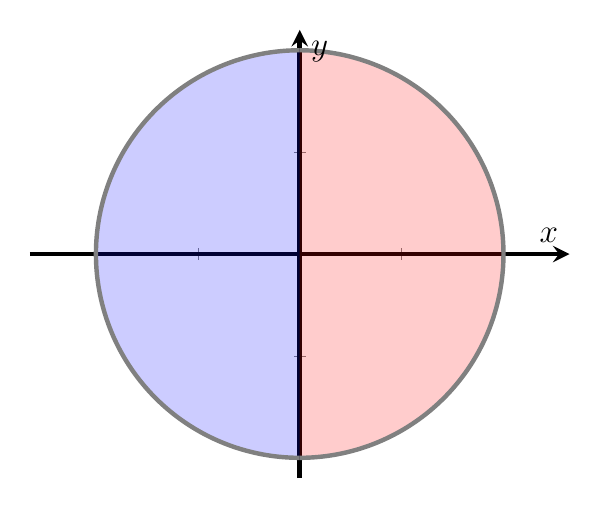
\begin{tikzpicture}
  \begin{axis} [
    Delta Style,
    xmin = -1.1,
    xmax =  1.1,
    ymin = -1.1,
    ymax =  1.1,
    xticklabels = {$ $,$ $,$ $,$ $,$ $,$ $,$ $,$ $,$ $},
    yticklabels = {$ $,$ $,$ $,$ $,$ $,$ $,$ $,$ $,$ $}
    ]

    \addplot [mark=none,gray, fill=red, fill opacity = 0.2, ultra thick, samples=200, domain=-0.5*pi:0.5*pi] ({cos(deg(x))}, {sin(deg(x))});
    
    \addplot [mark=none,gray, fill=blue, fill opacity = 0.2, ultra thick, samples=200, domain=0.5*pi:1.5*pi] ({cos(deg(x))}, {sin(deg(x))});
    % \node[gray] at (axis cs:-0.2,0.5){$x=0$};
    % \node[gray] at (axis cs: 0.7,0.5){$y = \sqrt{x}$};
    % \node[] at (axis cs: 1.2,0.5){$y=0$};
    % \node[] at (axis cs: 0.3,1.1){$y=1$};

  \end{axis}
\end{tikzpicture}
\end{document}